\begin{figure}[h!]
    \centering
    \begin{subfigure}[b]{0.23\textwidth}
        \centering
        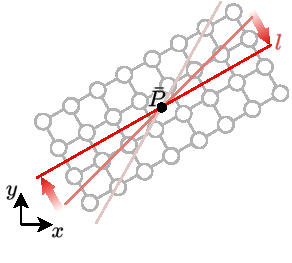
\includegraphics[width=\textwidth]{images/inert_0.drawio.svg.pdf}
        % \caption{}
        \label{fig:inert_1}
    \end{subfigure}
    \hfill
    \begin{subfigure}[b]{0.23\textwidth}
        \centering
        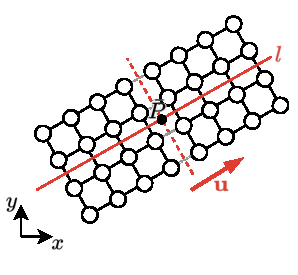
\includegraphics[width=\textwidth]{images/inert.drawio.svg.pdf}
        % \caption{}
        \label{fig:inert_2}
    \end{subfigure}
    \caption{Illustration of the inertial bisection in 2D: dividing the graph
    along the line orthogonal to the direction $\mathbf{u}$ through the center of mass $\bar{P}$ that minimizes the sum of squared distances.}
    \label{fig:inert}
\end{figure}